\section*{Appendix}
\subsection*{The choice of sampling radius}
The number of graph nodes and edges will influence the memory footprint and computational cost for the solver. The farthest point sampling method~\cite{moenning2003fast} is to repeatedly add the farthest point to the graph until the geodesic distance between graph nodes and the farthest point is smaller than the given radius parameter $R$. Compared with farthest point sampling method(Fig.~\ref{fig:diffsample}), our adopt method can obtain fewer nodes and is faster to converge with the similar accuracy. In our method, the radius $R$ can be used to balance the speed and accuracy. A smaller $R$ leads to more nodes in the deformation graph, which increases the number of variables and accuracy while requires more computational time. We show the comparison in Fig.~\ref{fig:diffr}. Our method does not vary the sampling density based on curvature. In our experiments, such uniform density is sufficient to generate good results and curvature-adaptive sampling can be a future work.

\begin{figure}[!htb]
    \centering
    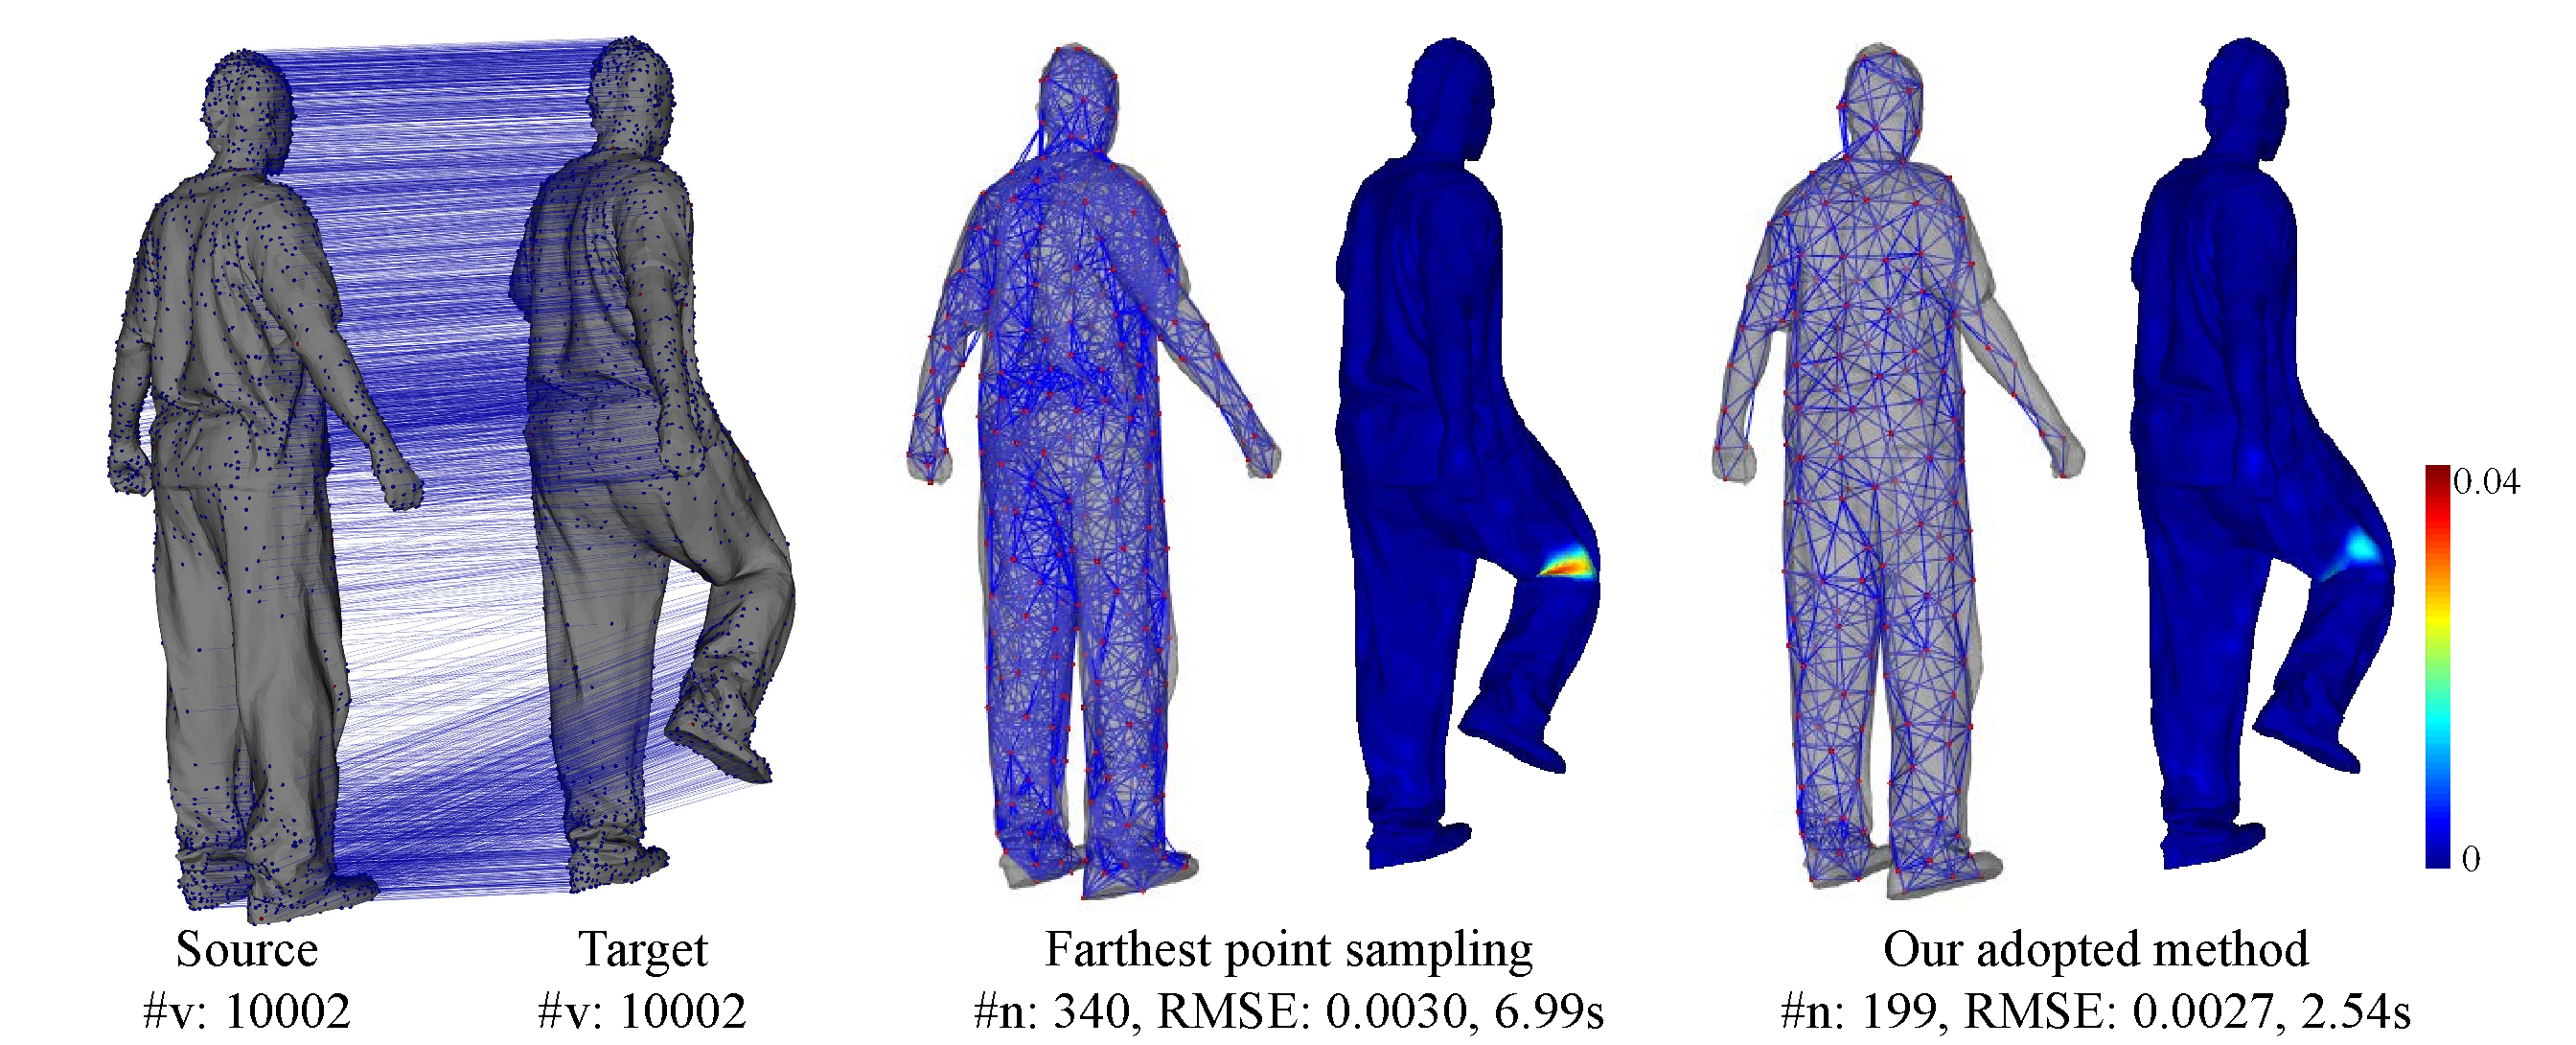
\includegraphics[width=0.95\columnwidth]{Figs/diffsample.pdf}
    \caption{Comparison with the farthest sampling method for the given radius $R=5\overline{l}$, where $\overline{l}$ is the average edge length on the source surface. The farthest point sampling method can obtain more graph nodes.($k_{\alpha}=0.001, k_{\beta}=0.1$). The RMSE and the color-coded registration errors are in the unit of meters.}
    \label{fig:diffsample}
\end{figure}


\begin{figure}[!htb]
    \centering
    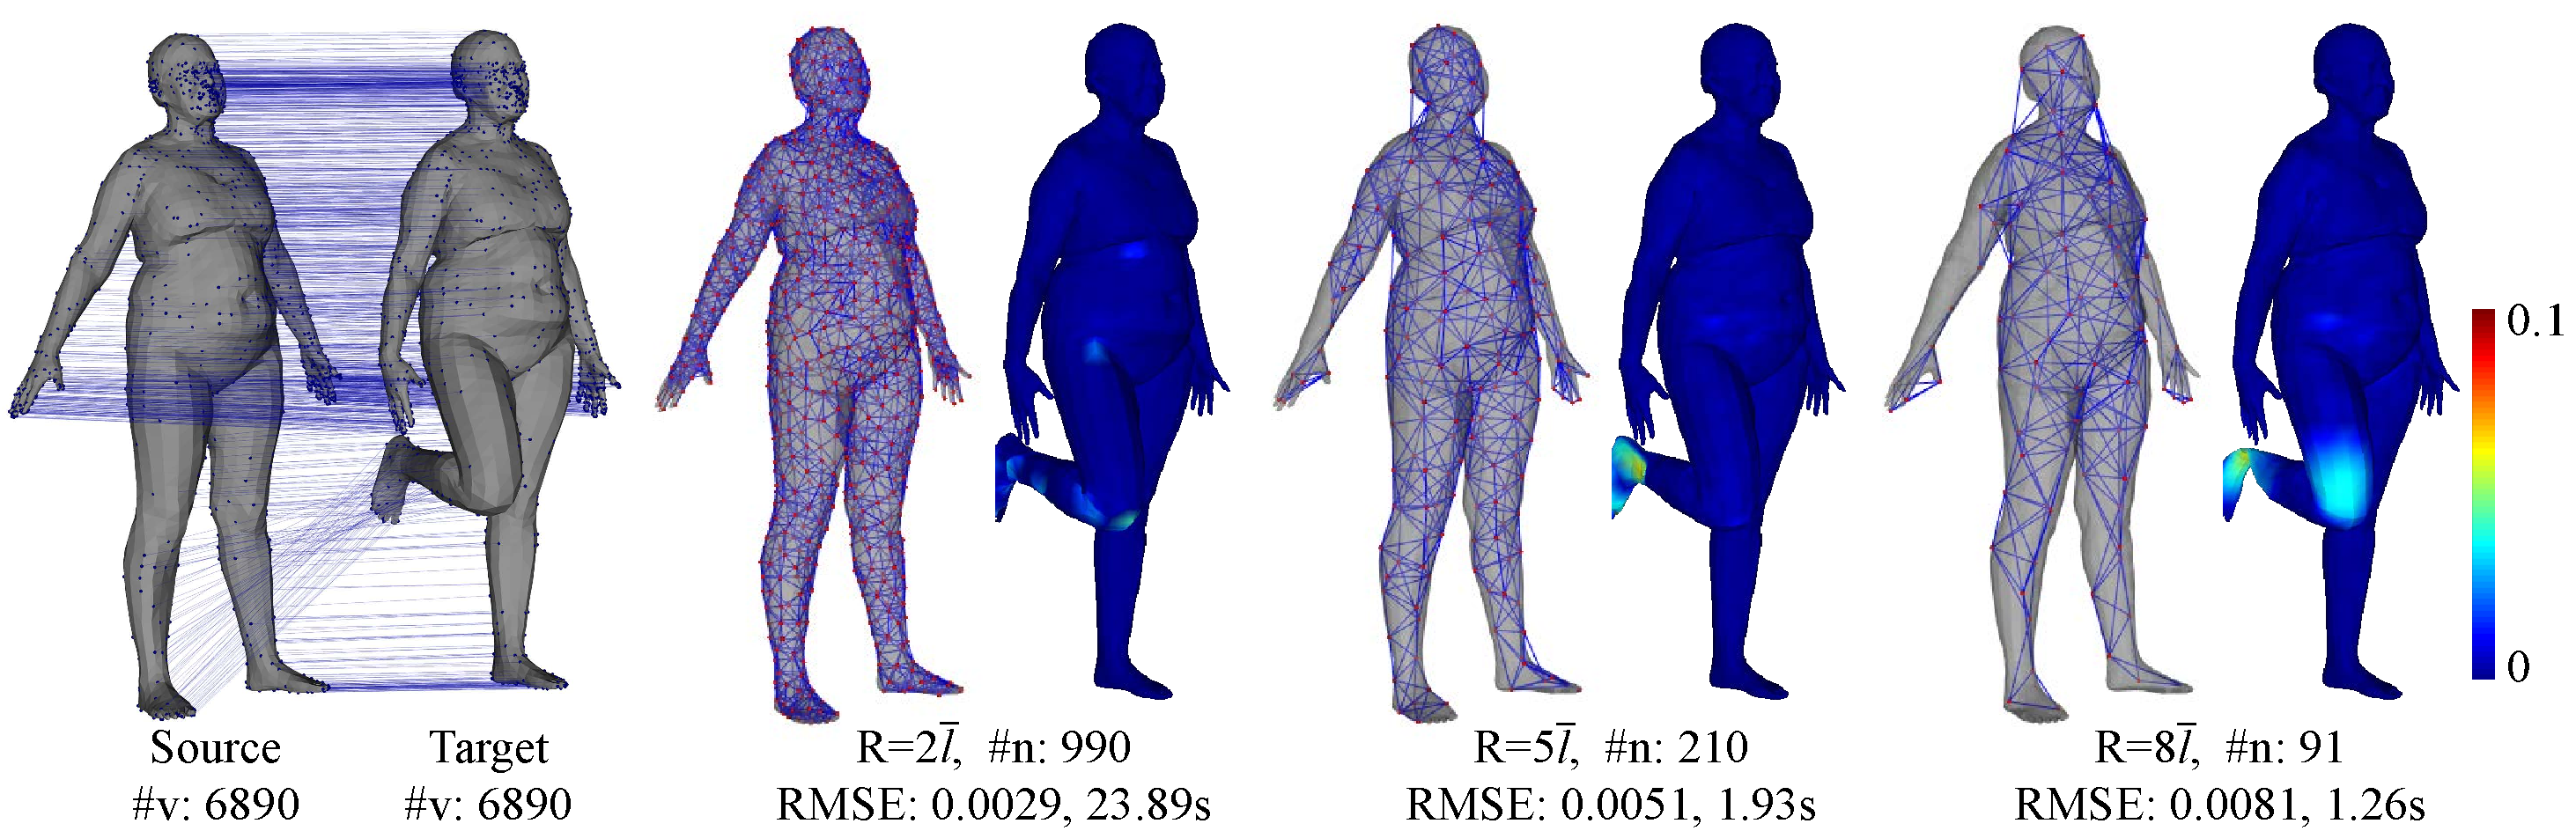
\includegraphics[width=\columnwidth]{Figs/diffr.pdf}
    \caption{Comparison with different sampling radius with $k_{\alpha}=0.001, k_{\beta}=0.1$. More nodes can get more accurate results. The RMSE and the color-coded registration errors are in the unit of meters.}
    \label{fig:diffr}
\end{figure}


\subsection*{The comparison with fixed parameters}
In our method, the $\nua$ and $\nur$ values will influence the registered result, and discussion on this part is given in "Choosing $\nua$ and $\nur$"(Sec 4.2) of the paper. In Fig.~\ref{fig:fixnu}, we show the comparison between our dynamic adjustment strategy and the strategy by fixing $\nua, \nur$, and we can see our method can get higher accuracy.
\begin{figure}[!htb]
    \centering
    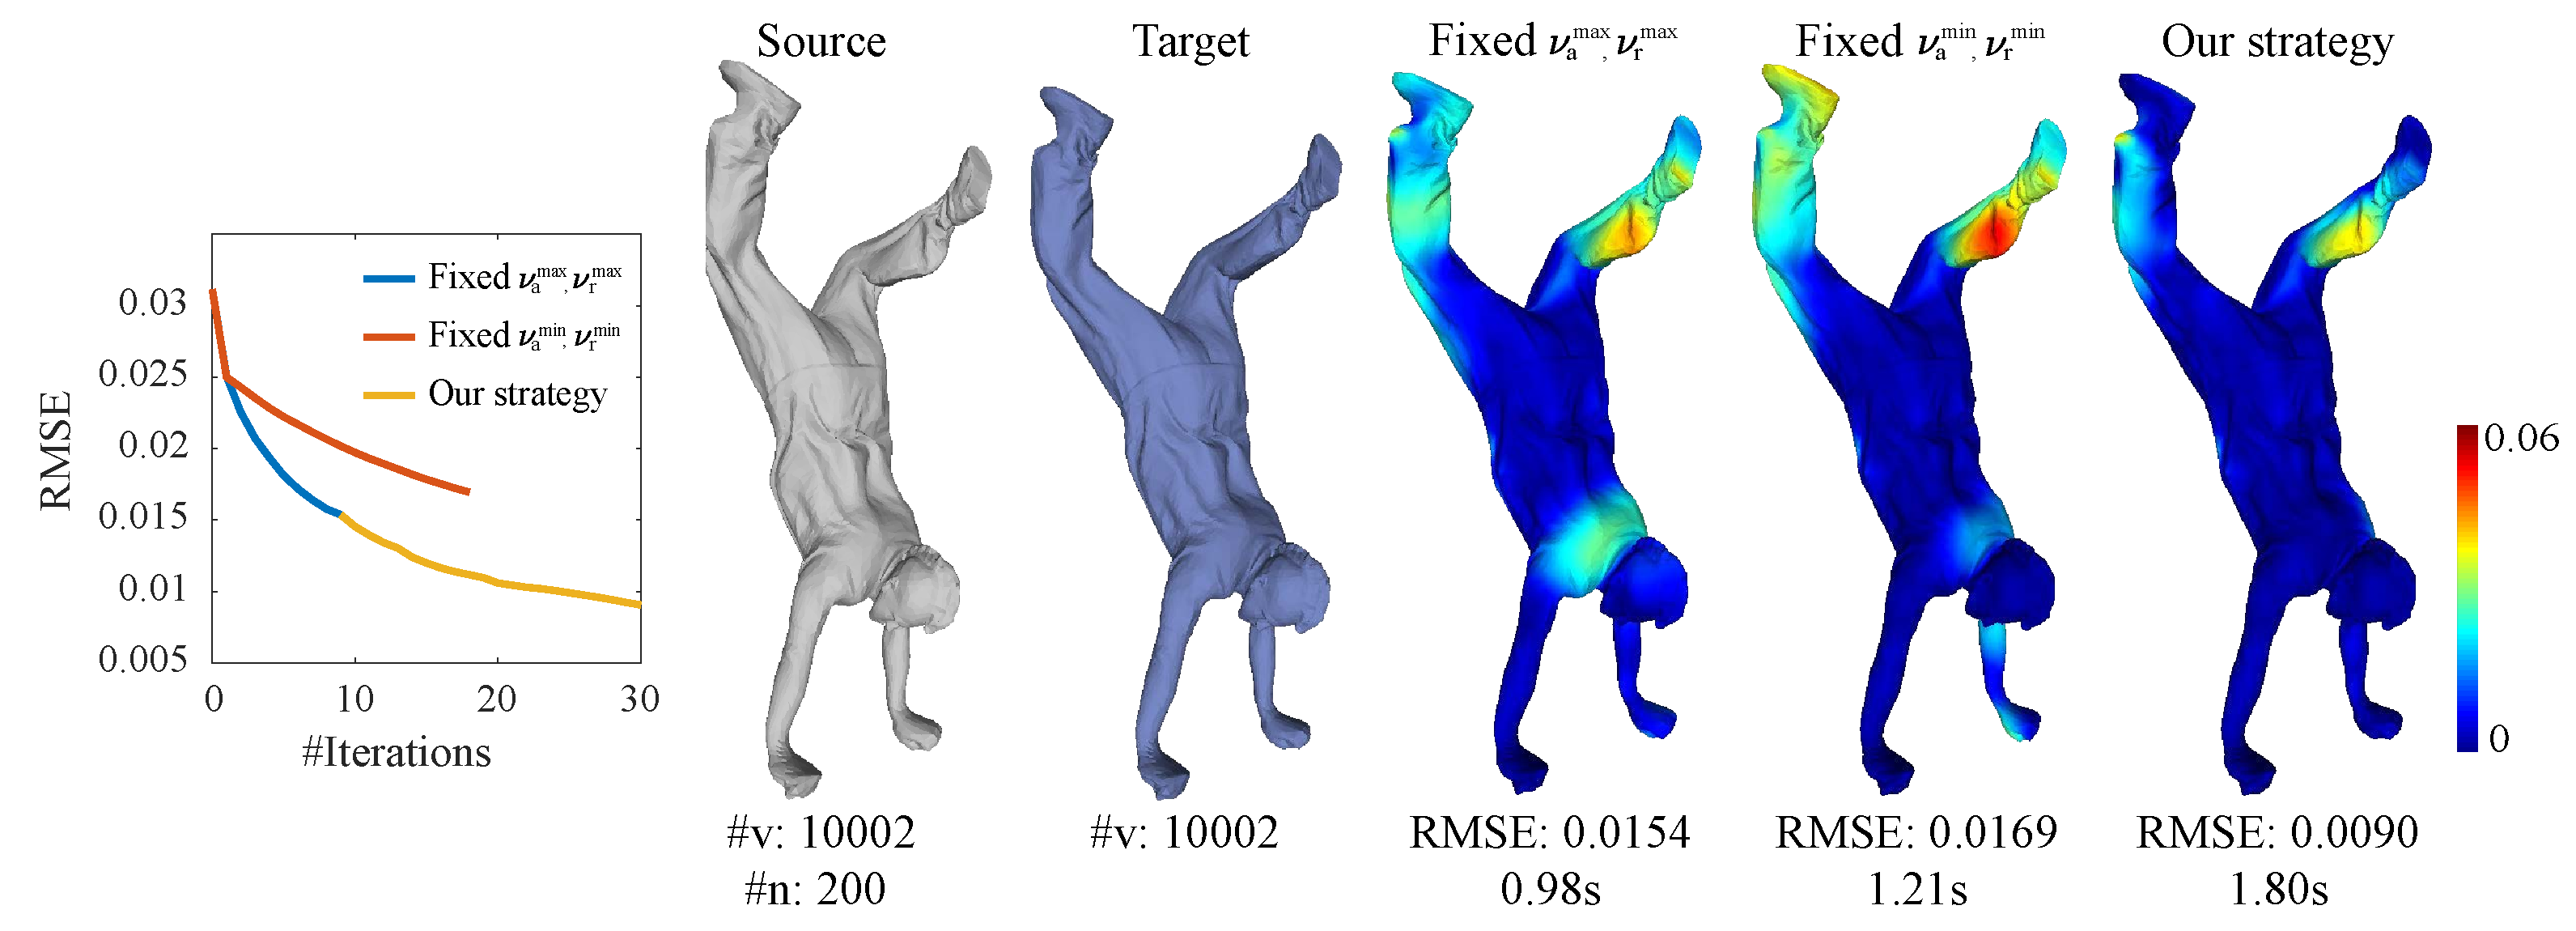
\includegraphics[width=1\columnwidth]{Figs/fixednu.pdf}
    \caption{Comparison with fixed $\nua, \nur$ on 42-th to 40-th mesh in "handstand" with $k_{\alpha}=100$ and $k_{\beta}=50$. Here $\nur^{\min}$ is the value when $\nua$ reaches $\nua^{\min}$. The RMSE and the color-coded registration errors are in the unit of meters.}
    \label{fig:fixnu}
\end{figure}

\begin{figure*}[b]
    \centering
     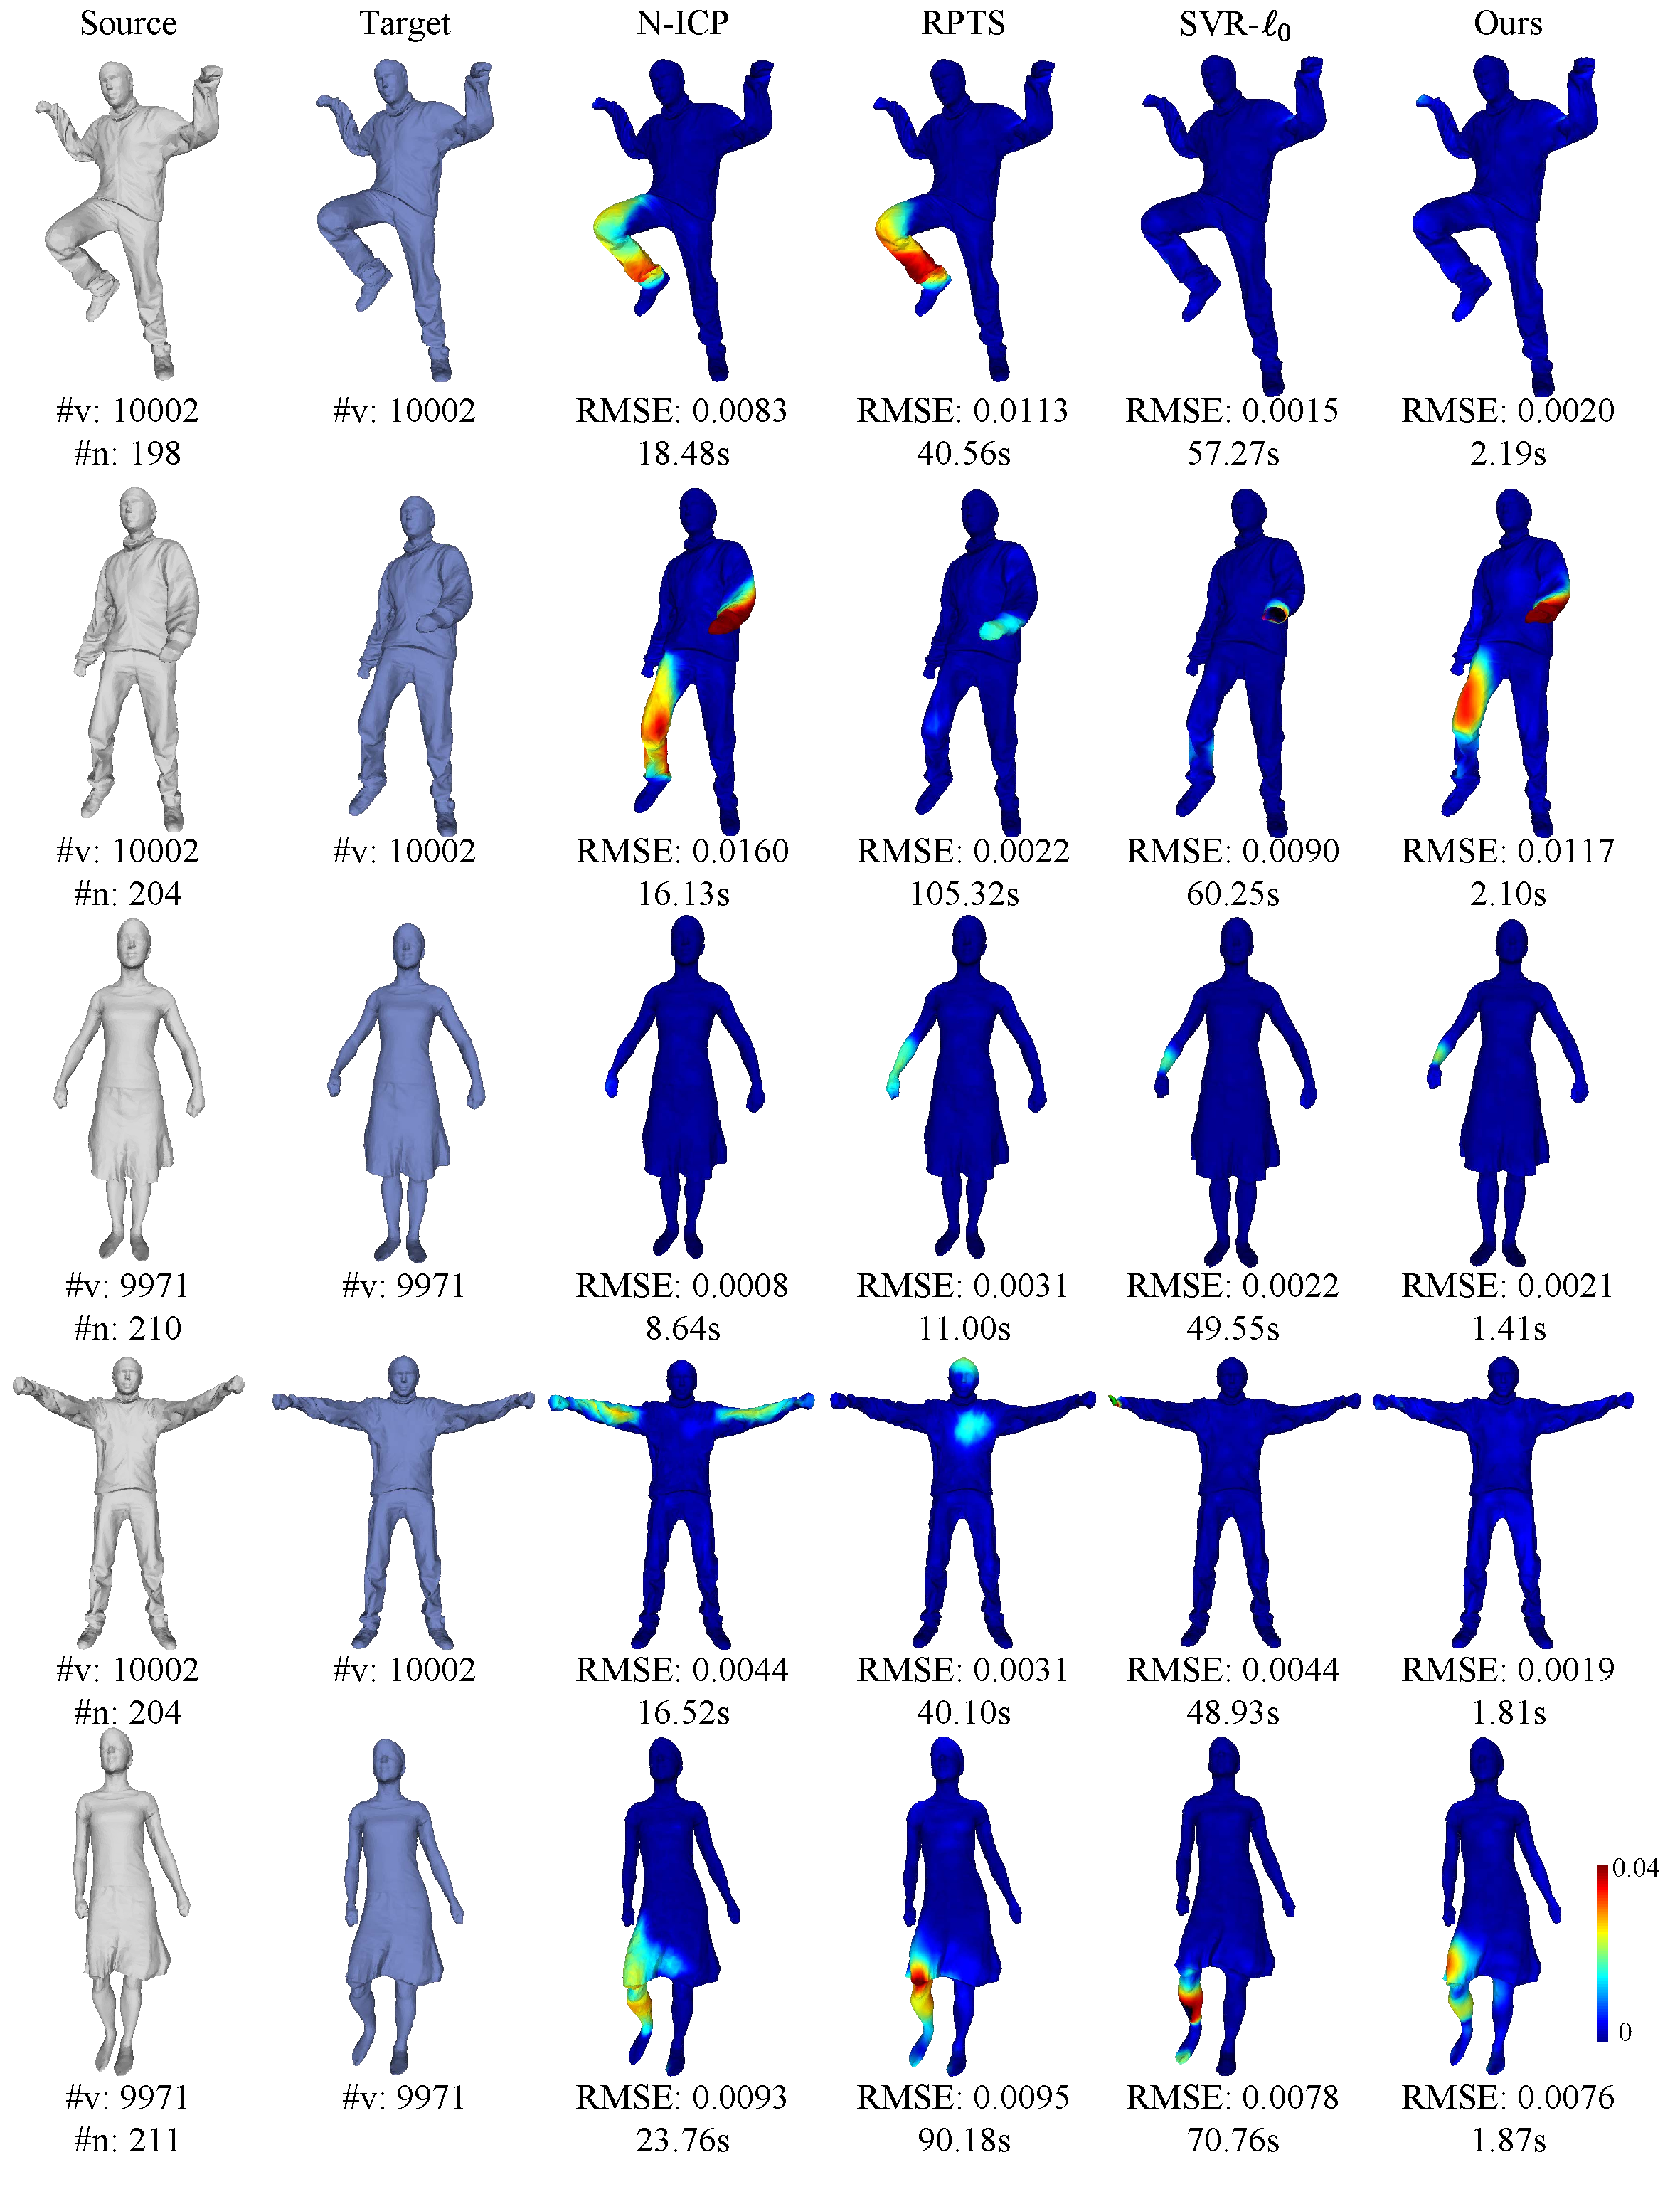
\includegraphics[width=\textwidth]{Figs/supp_clean.pdf}
    \caption{Comparison with N-ICP, RPTS and SVR-$\ell_0$ on ``crane'', ``march1'', ``samba'', ``squat1'' and ``swing'' datasets with small deformation. We set $\alpha = 10$ for N-ICP, $\alpha = 10$ and $\beta = 1$ for RPTS, $\alpha = 0.1$ and $\beta = 100$ for SVR-$\ell_0$, and $k_{\alpha} = 1, k_{\beta} = 10^3, \nua=30\overline{l}$ for our method in these examples. The RMSE and the color-coded registration errors are in the unit of meters.}
\label{fig:small}
\end{figure*}

\subsection*{Experiment on clean data}
We show more results on five models ``crane'', ``march1'', ``samba'', ``squat1'' and ``swing'' in Human-motion datasets. For each model, we use the closest points to construct the correspondences for small deformation, and use the SHOT with diffusion pruning method for big deformation. For each method, we search the parameter setting for best performance. The results are shown in Fig.~\ref{fig:small} and Fig.~\ref{fig:big}, and we can see that our method is faster than other methods and achieves similar or better accuracy.
\begin{figure*}[b]
    \centering
     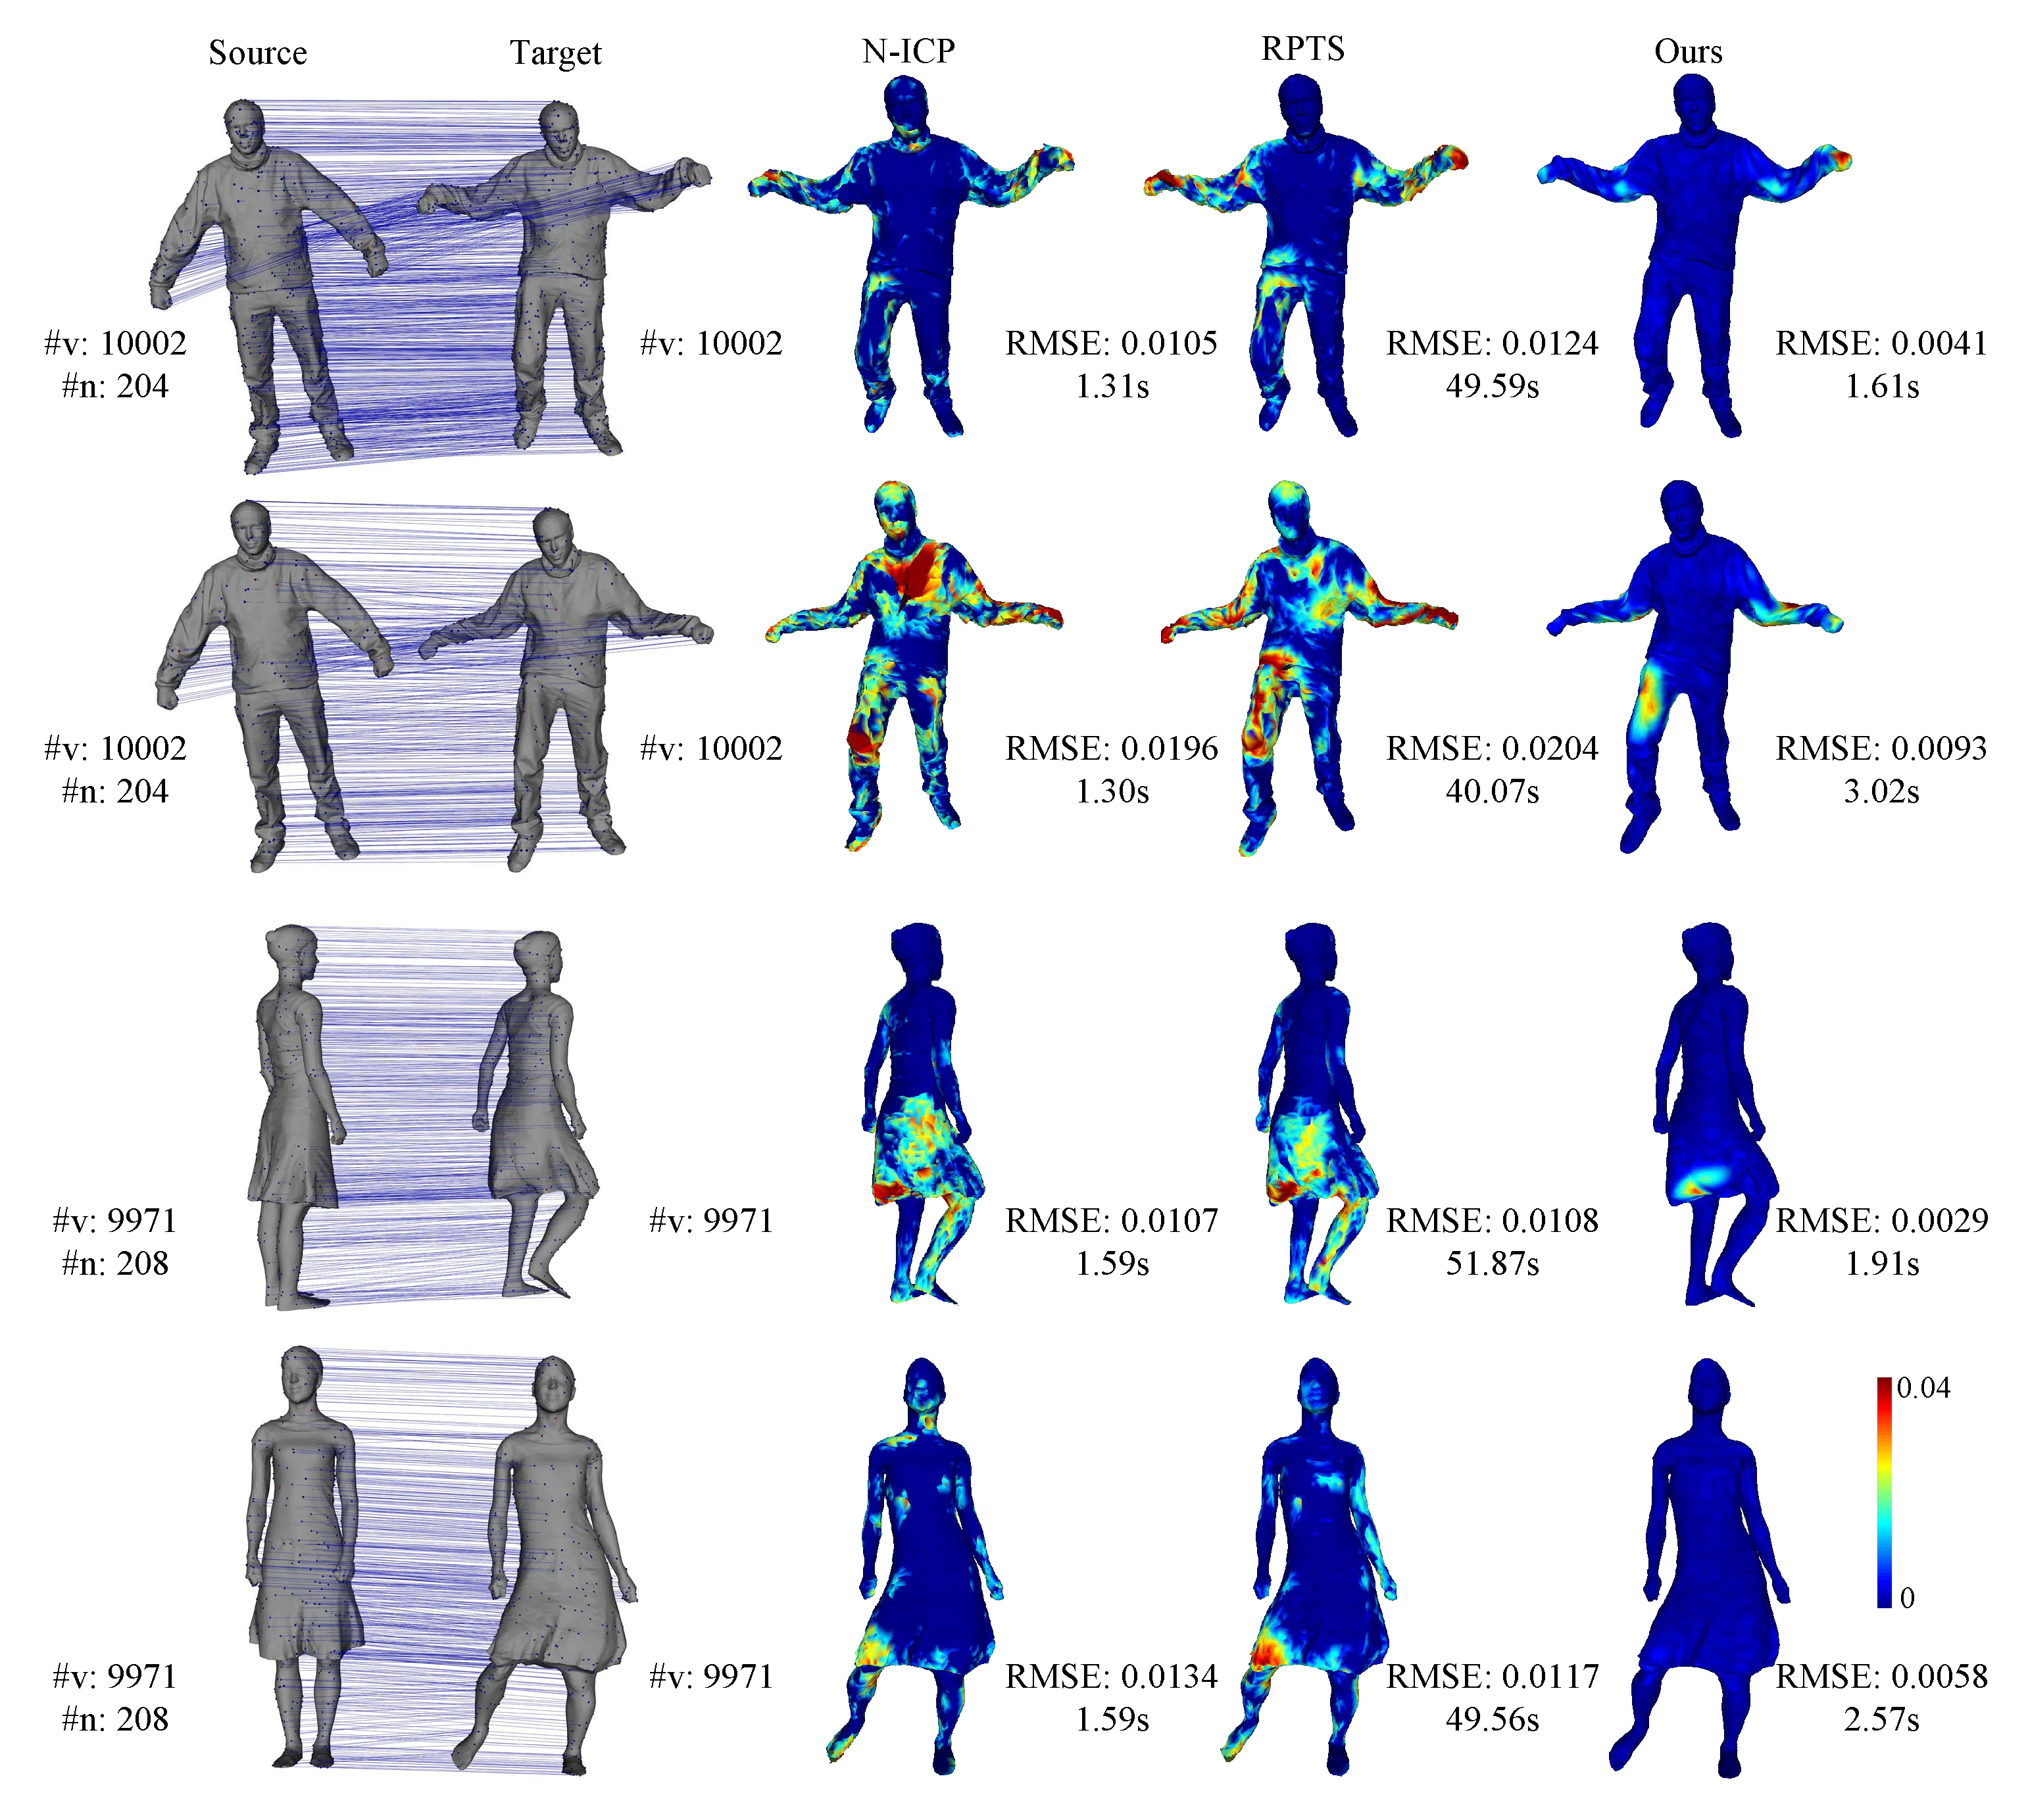
\includegraphics[width=\textwidth]{Figs/supp_clean2.pdf}
    \caption{Comparison with N-ICP, RPTS and SVR-$\ell_0$ on ``crane'',and ``swing'' datasets with big deformation. We set $\alpha = 0.01$ for N-ICP, $\alpha = 0.01$ and $\beta = 1$ for RPTS, and $k_{\alpha} = 0.01$ and $k_{\beta} = 1$ for our method in these examples. The RMSE and the color-coded registration errors are in the unit of meters.}
\label{fig:big}
\end{figure*}

\subsection*{Experiment on partially overlapping data}
We show more results and comparisons on partially overlapping data from ``bouncing'' datasets. We choose $\alpha = 10$ for N-ICP, $\alpha = 1, \beta = 100$ for RPTS, $\alpha = 0.1, \beta = 100$ for SVR-$\ell_0$, and $k_{\alpha} = 1, k_{\beta} = 100, \nua^{\max}=30\overline{d}, \nur^{\max}=100\overline{l}$ for our method and $\theta=45^{\circ}$ for all method in these examples. The results are shown in Fig.~\ref{fig:partial}, and we can see that our methods is robust to partially overlapping data, and faster than other methods.
\begin{figure*}[h]
    \centering
     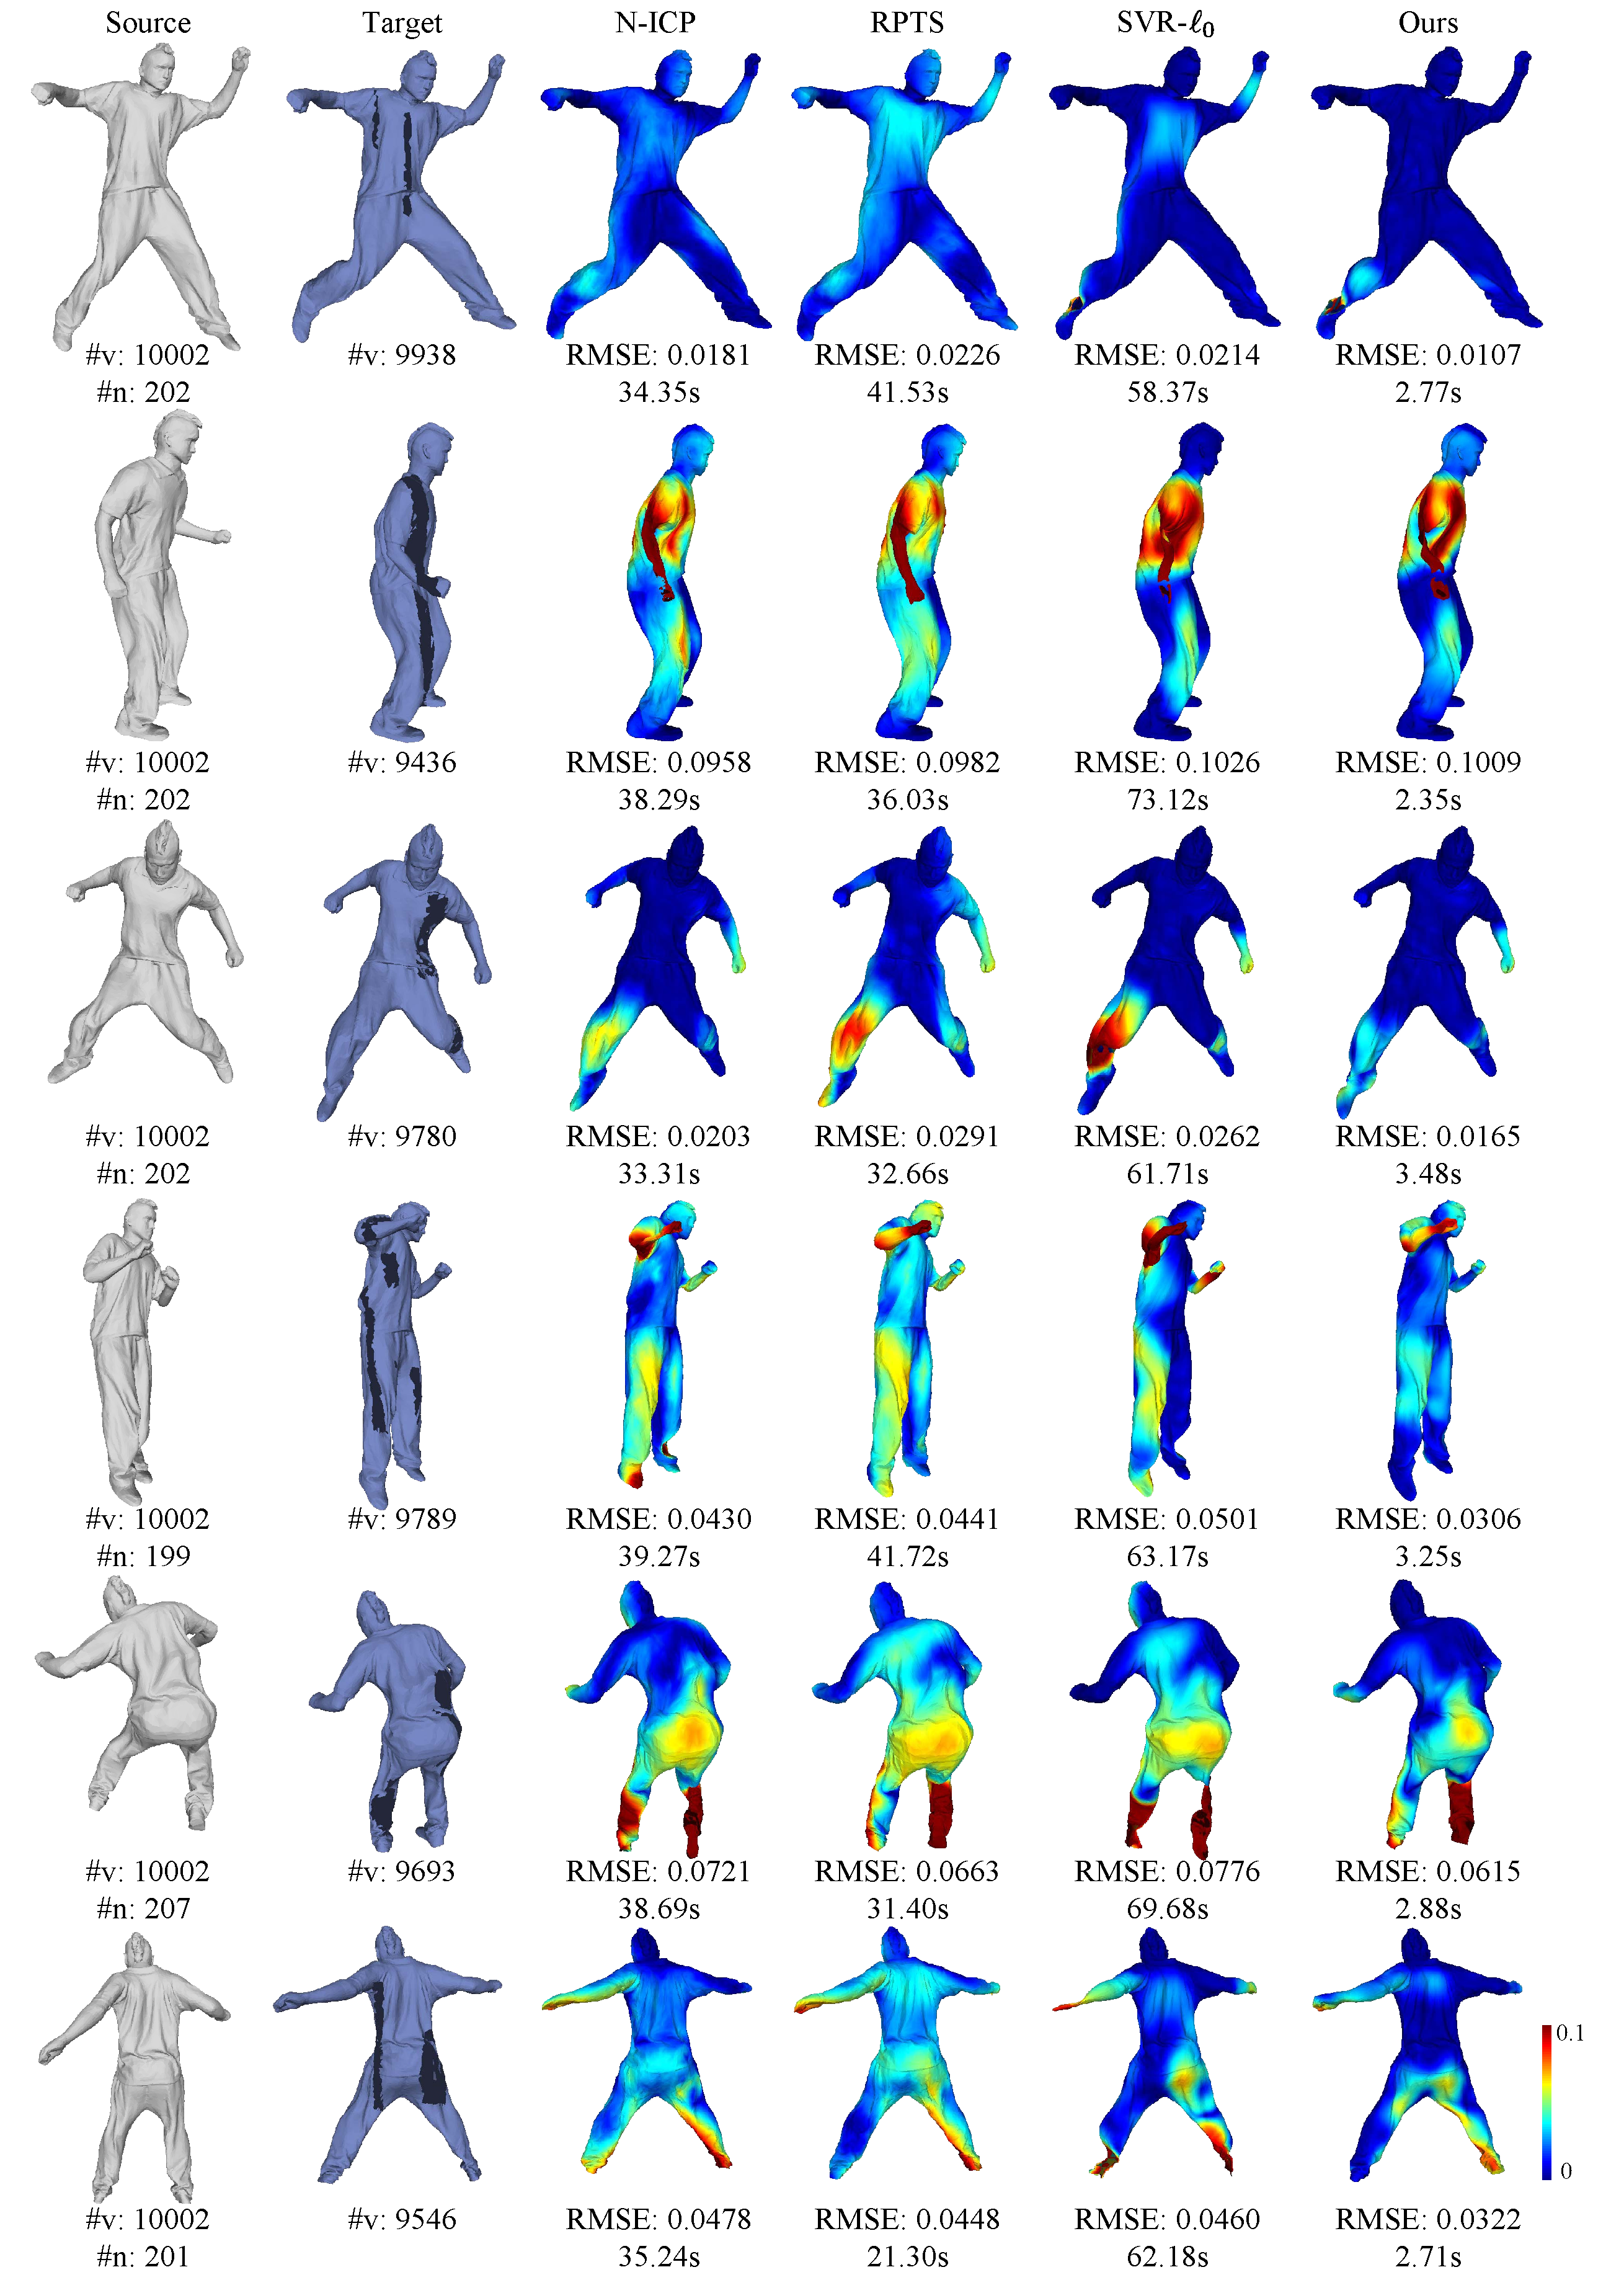
\includegraphics[width=0.9\textwidth]{Figs/supp_partial.pdf}
    \caption{Comparison with N-ICP, RPTS and SVR-$\ell_0$ on ``bouncing''  datasets with partially overlapping data. The RMSE and the color-coded registration errors are in the unit of meters.}
    \label{fig:partial}
\end{figure*}